\documentclass[dvipsnames]{standalone}

\usepackage{tikz}
\usetikzlibrary{shapes, arrows, positioning,backgrounds,scopes}
\usepackage{xcolor}


\pgfdeclarelayer{background}
\pgfsetlayers{background,main}

\definecolor{lightturkis}{HTML}{03bdeb}
\definecolor{turkis}{HTML}{2cb1d2}
\definecolor{darkturkis}{HTML}{4ca2b8}

\definecolor{lightblue}{HTML}{3011e3}
\definecolor{blue}{HTML}{4d37ca}
\definecolor{darkblue}{HTML}{6154b0}

\definecolor{lightpurple}{HTML}{9e03e6}
\definecolor{purple}{HTML}{992bcc}
\definecolor{darkpurple}{HTML}{924ab3}

\definecolor{lightorange}{HTML}{FFA364}
\definecolor{orange}{HTML}{FF6802}
\definecolor{darkorange}{HTML}{9C3F00}

\newcommand{\odmlbuntraw}{
	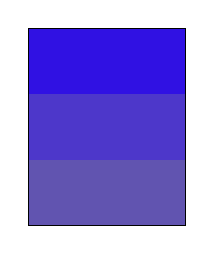
\begin{tikzpicture}
	    \begin{scope}[scale=0.5]
		\draw[darkblue,fill=darkblue]  (0,0) rectangle (4,5/3);
		\draw[blue,fill=blue]  (0,5/3) rectangle (4,10/3);
		\draw[lightblue,fill=lightblue]  (0,10/3) rectangle (4,15/3);
		\draw  (0,0) rectangle (4,5);
	    \end{scope}
	\end{tikzpicture}}
	
\newcommand{\odmltext}[2][below]{
	\begin{tikzpicture}
		\node(r) {\odmlraw};
		\node[align=center, #1= -0.3em of r] (t) {#2};
	\end{tikzpicture}}

\newcommand{\odmlbunttext}[2][below]{
	\begin{tikzpicture}
	\node(r) {\odMLtree};
	\node[align=center, #1= -0em of r] (t) {#2};
	\end{tikzpicture}}


\newcommand{\odMLtree}{
	\usetikzlibrary{positioning}
	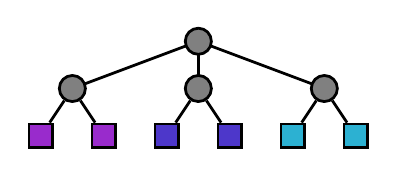
\begin{tikzpicture}
	\begin{scope}[scale=0.4]
	\node (State0) [-,circle, radius=0.8cm, draw=Black, fill=Gray, growth parent anchor=south] {} [-, line width=1, sibling distance=4cm]
	    child{ [sibling distance=2cm]
		  node (State00) [circle, radius=0.8cm, draw=Black, fill=Gray] {} 
		  child{node (State000) [rectangle, draw=Black, fill=purple, minimum width=0.3cm, minimum height=0.3cm] {}}
		  child{node (State001) [rectangle, draw=Black, fill=purple, minimum width=0.3cm, minimum height=0.3cm] {}}
	    }
	    child{ [sibling distance=2cm]
		  node (State01) [circle, radius=0.8cm, draw=Black, fill=Gray] {}
		  child{node (State011) [rectangle, draw=Black, fill=blue, minimum width=0.3cm, minimum height=0.3cm] {}}
		  child{node (State011) [rectangle, draw=Black, fill=blue, minimum width=0.3cm, minimum height=0.3cm] {}}
	    }
	    child{ [sibling distance=2cm]
		  node (State02) [circle, radius=0.8cm, draw=Black, fill=Gray] {}
		  child{node (State021) [rectangle, draw=Black, fill=turkis, minimum width=0.3cm, minimum height=0.3cm] {}}
		  child{node (State021) [rectangle, draw=Black, fill=turkis, minimum width=0.3cm, minimum height=0.3cm] {}}
	    };
	\end{scope}
	\end{tikzpicture}}
	
	
\begin{document}
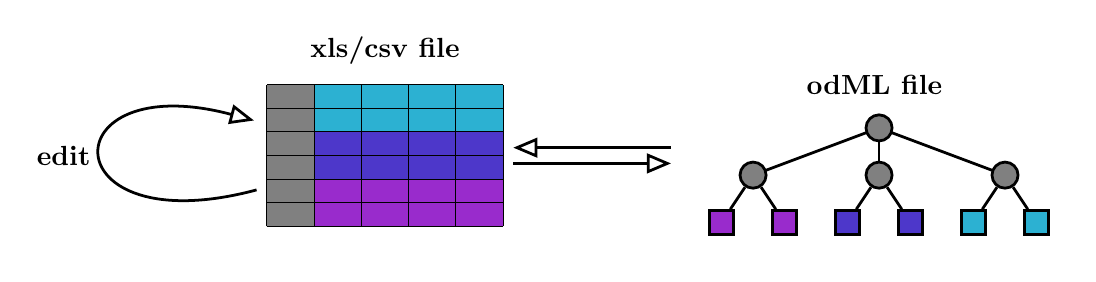
\begin{tikzpicture}
    \begin{scope}[scale=1]

    \node[](odml) {\odmlbunttext[above]{\textbf{odML file}}};
 

     \node[left = 2cm of odml] (table) {\tikz{
     \begin{scope}[scale=0.6]
	\path[fill=Gray] (-2,1) rectangle ++(1.0,-3);
	\path[fill=purple] (-1,-2) rectangle ++(4.0,0.5);
	\path[fill=purple] (-1,-1.5) rectangle ++(4.0,0.5);
	\path[fill=blue] (-1,-1) rectangle ++(4.0,0.5);
	\path[fill=blue] (-1,-0.5) rectangle ++(4.0,0.5);
	\path[fill=turkis] (-1,0) rectangle ++(4.0,0.5);
	\path[fill=turkis] (-1,0.5) rectangle ++(4.0,0.5);
% 	\path[fill=blue] (-1,1) rectangle ++(4.0,0.5);
% 	\path[fill=darkblue] (-1,1.5) rectangle ++(4.0,0.5);
	\draw[xstep=1,ystep=0.5] (-2,-2) grid (3,1);
    \end{scope}
    }};
% 
    \node[above = 0cm of table](tabletext) {\textbf{xls/csv file}};
% 
    \draw[-open triangle 45, line width=1] ([yshift=0.1cm]odml.west) -- ([yshift=0.1cm]table.east) {};
    \draw[-open triangle 45, line width=1] ([yshift=-0.1cm]table.east) -- ([yshift=-0.1cm]odml.west) {};
    \path (table) edge  [>=open triangle 45,loop left, line width=1] node {\textbf{edit}} ++ (0.1,0);
    \end{scope}
\end{tikzpicture}
\end{document}
